\documentclass[compress,10pt]{beamer}
% version imprimable pour assistance
%\documentclass[10pt, green, handout]{beamer}
\usepackage[T1]{fontenc}
\usepackage[utf8]{inputenc}
\usepackage[frenchb]{babel} % le document est en français
\usepackage{rotating,amsmath}
\usepackage{graphicx,cancel}       % pour ins\'erer des figures
        % pour d\'efinir plus de couleurs
\usetheme{Malmoe}  %Applique le theme INRA (ce dernier doit être present dans le repertoire courant)
\usepackage{xcolor,colortbl}
\usepackage{array}
\usepackage{mdframed}
\usepackage{listings}
\usepackage{lmodern}	
\usepackage{tikz}
\usetikzlibrary{positioning,shapes,arrows}


\definecolor{lgreen}{RGB}{188,214,49}
\definecolor{dgreen}{RGB}{139,172,33}
%\setbeamercolor{structure}{fg=INRA@dinst}

\setbeamertemplate{blocks}[rounded][shadow=true]
\setbeamercolor{block title}{use = structure , fg=dgreen, bg = dgreen!35}
\setbeamercolor{normal text}{fg=black,bg=white}
\setbeamercolor{alerted text}{fg=lgreen}
\setbeamercolor{example text}{fg=lgreen}
\setbeamercolor{structure}{fg=dgreen} %d'où ce bleu par défaut
\setbeamercolor{background canvas}{parent=normal text}


 \usepackage{tikz}

\usetikzlibrary{calc,shapes,backgrounds,arrows,automata,shadows,positioning}



\addtobeamertemplate{navigation symbols}{}{%
    \usebeamerfont{footline}%
    \usebeamercolor[fg]{footline}%
    \hspace{1em}%
    \insertframenumber/\inserttotalframenumber
}
%\pgfdeclareimage[height=\paperheight,width=\paperwidth]{intro}{plots/plante-insecte-ombre-COLLAGE.jpg}
%\setbeamertemplate{background canvas}{\pgfuseimage{intro}}

%\newmdenv[tikzsetting={draw=black, fill=white, fill opacity =0.7, line width= 4pt}, backgroundcolor=white, leftmargin=0, rightmargin=40,innertopmargin=4pt]{titlebox}


\setbeamertemplate{frametitlecontinuation}{\insertcontinuationcountroman}

%-------------------------------------------------------------------------------
% Quelques options pdf
%-------------------------------------------------------------------------------
\hypersetup{
pdfpagemode = FullScreen, % afficher le pdf en plein \'ecran
pdfauthor   = {},%
pdftitle    = {},%
pdfsubject  = {},%
pdfkeywords = {Science,Impact},%
pdfcreator  = {PDFLaTeX,emacs,AucTeX},%
pdfproducer = {INRA}%
}


\newcommand\Wider[2][3em]{%
\makebox[\linewidth][c]{%
  \begin{minipage}{\dimexpr\textwidth+#1\relax}
  \raggedright#2
  \end{minipage}%
  }%
}

\AtBeginSection[]
{  \begin{frame}
  \frametitle{}
  \tableofcontents[currentsection, hideothersubsections]
  \end{frame} 
}



%
\newcommand{\bX}{\boldsymbol{X}}

\newcommand{\Xall}{\bX}
\newcommand{\Zall}{\bZ}
\newcommand{\M}{\mathcal{M}_{K_0,K_1,\dots, K_Q}}
\newcommand{\ind}{\mathds{1}}

\newcommand{\Mcal}{\mathcal{M}}


\newcommand{\bZ}{\boldsymbol{Z}}
\newcommand{\bpi}{\boldsymbol{\pi}}
\newcommand{\balpha}{\boldsymbol{\alpha}}
\newcommand{\btau}{\boldsymbol{\tau}}


\def\Ecal{\mathcal{E}}



\def\N{\mathbb{N}}
\def\R{\mathbb{R}}
\def\F{\mathcal{F}}
\def\Nb{\boldsymbol{N}}
\def\bZ{\boldsymbol{Z}}
\def\btheta{\boldsymbol{\theta}}
\def\bpi{\boldsymbol{\pi}}
\def\bY{\boldsymbol{Y}}
\def \ind{\mathbb{I}}
\def \P{\mathbb{P}}
\def \vert{\color{dgreen}}

\def \rouge{\color{red}}
\def \noir{\color{black}}
%-------------------------------------------------------------------------------
\title[Formation Réseaux 06/2019]{ Données de réseaux : introduction }
%\subtitle{}
\author[Donnet, Massol, Verzelen]{ Sophie Donnet, François Massol, Nicolas Verzelen\\ MIA Paris, INRA, CNRS}
\titlegraphic{
\includegraphics[width=2cm]{plots/logoINRA.png}
}
\date{Formation Réseaux MIRES / ReSodiv / COEX\\ 18-19-06/2019}
%-------------------------------------------------------------------------------
\begin{document}




%-F1------------------------------------------------------------------------------
\begin{frame}
\titlepage
\end{frame}

\setbeamertemplate{background canvas}[default]

\begin{frame}
Tous les documents seront disponibles à cette adresse 

\url{https://github.com/Sophiedonnet/Formation_Reseau_MIRES}

\end{frame}

\section[Contexte]{Contexte}

%-------------------------------------------------------------------------------

\begin{frame}{Pourquoi un réseau?}

\begin{itemize}
\item Etudier/comprendre un \textcolor{dgreen}{certain type de  relations} entre des 
\textcolor{dgreen}{acteurs donnés}
\item \textbf{Examples}
\begin{itemize}
\item Dons de semences de riz entre agriculteurs de riz au Vietnam
\item Relations d'amitiés entre agriculteurs au Vanuatu
\item Relations de co-occurence entre espèces animales dans un ecocystème donné
\item Inventaires de culture : relations entre agricultures et des espèces. 
\item Relation de pollinisation entre espèces animales et espèces végétales
\end{itemize}
\end{itemize}
\end{frame}

%------------------------------------------------------------------------------ 


\section{Des données terrains au réseau}

\begin{frame}{Définition d'un réseau}

\begin{block}{Définition}

Un réseau est la donnée d'un ensemble de noeuds (ou sommets) et d'arêtes entre ces sommets.

\begin{itemize}
\item  Un réseau est spécifique à \emph{un type de relation fixé}. 
\item  Les noeuds représentent des agents / individus / espèces animales
\item  Une arête existe entre deux sommets si ces deux agents ont une relation. 
\end{itemize}
\end{block}
\centering
 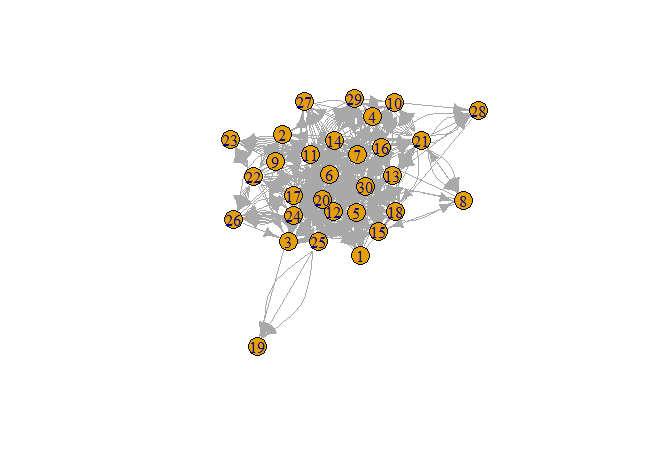
\includegraphics[width = 5cm]{plots/Vanuatu_directed.png} 
\end{frame}

%-------------------------------------------------------------------------------
\begin{frame}{Du terrain à l'objet réseau}

\begin{itemize}
\item  Partant des interviews  ou des relevés de terrain... 

\begin{tabular}{cc}
  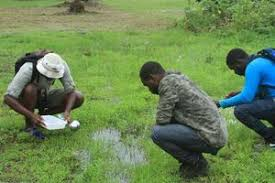
\includegraphics[width = 0.3 \textwidth, height=2cm]{plots/eco_1.jpg} &
 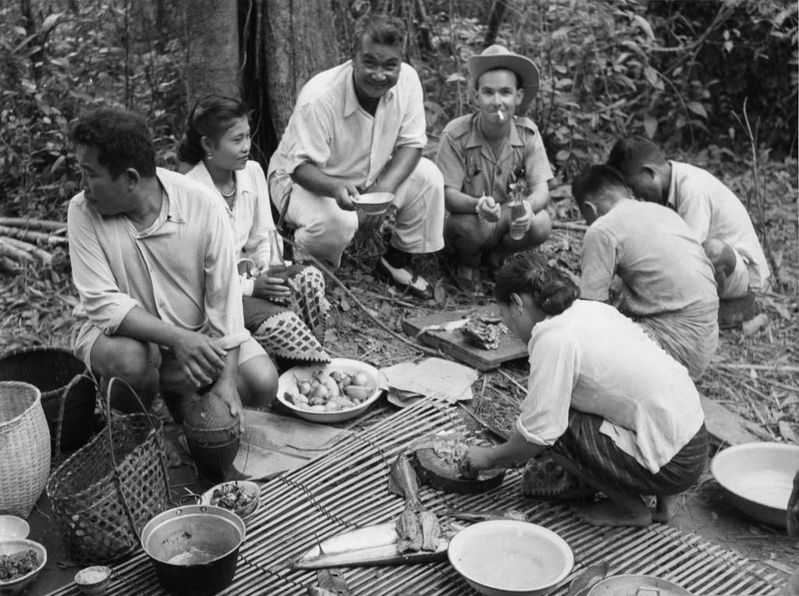
\includegraphics[width = 0.3 \textwidth, height=2cm]{plots/ethno_2.jpg}
% 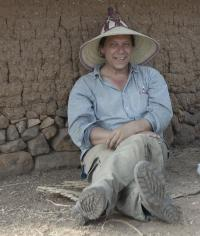
\includegraphics[width = 3cm]{plots/ethno_3.jpg}
\end{tabular}
\item ... on recupère des notes... 
\begin{tabular}{c}
 
\includegraphics[width = 0.3 \textwidth, height=2cm]{plots/tas_notes.jpg} 
\end{tabular}
\item ... qu'on transforme en fichier excel

\begin{tabular}{c}
 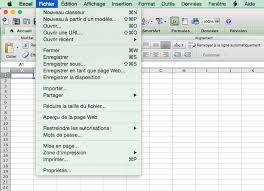
\includegraphics[width = 0.3 \textwidth, height=2cm]{plots/excel.jpg} 
\end{tabular}
\end{itemize}


\end{frame}

%------------------------------------------------------------------------------ 
\begin{frame}{Un exemple de données terrain}


\begin{itemize}
\item Données de E. Pannier (IRD, UMR 208 Paloc)
\item Circulation de variétés de riz au VietNam. 
\item Naturellement:  liste des échanges \emph{ayant eu lieu}
\end{itemize}
 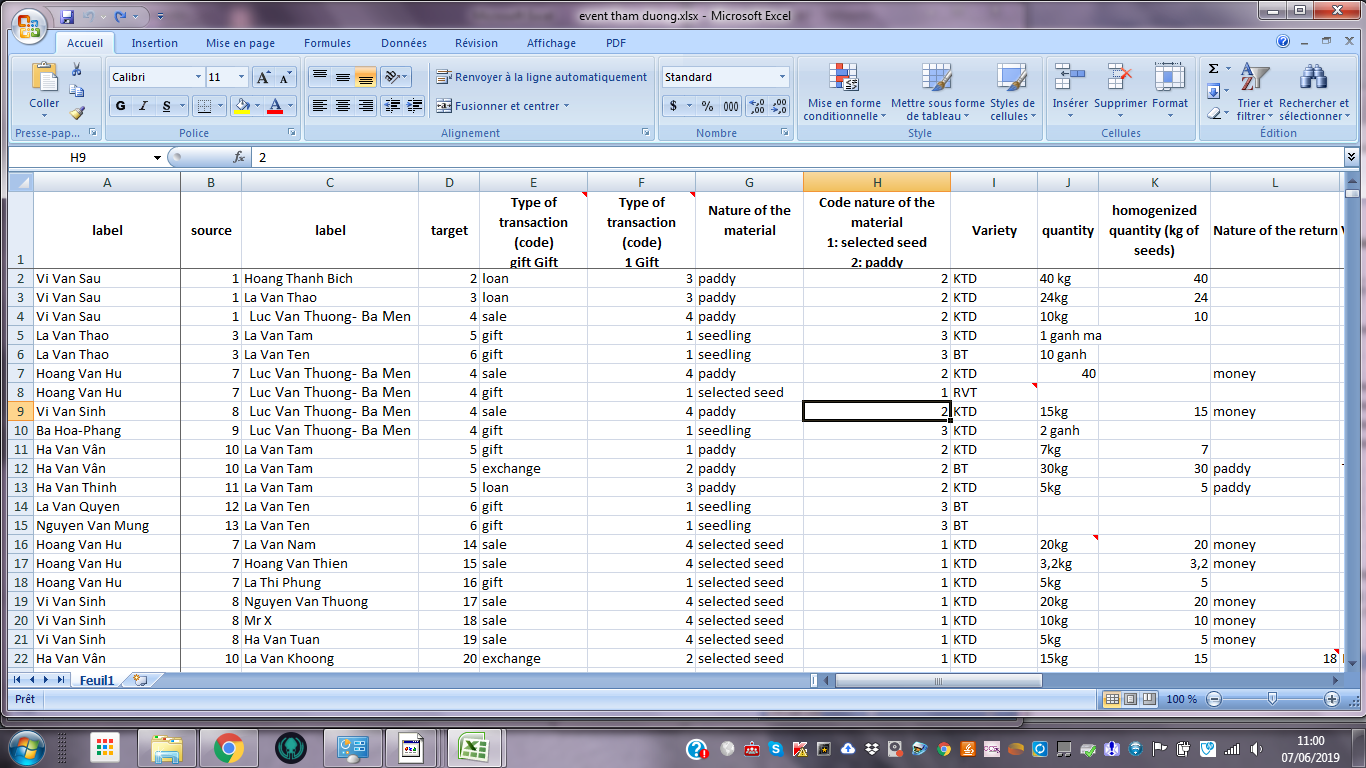
\includegraphics[width =  \textwidth]{plots/data_pannier_reseau.png} 
\end{frame}
%------------------------------------------------------------- 

\begin{frame}{Représentation du réseau}
\begin{itemize}
\item Liste des échanges : liste des arêtes
\item Suffisant pour décrire et tracer le réseau


 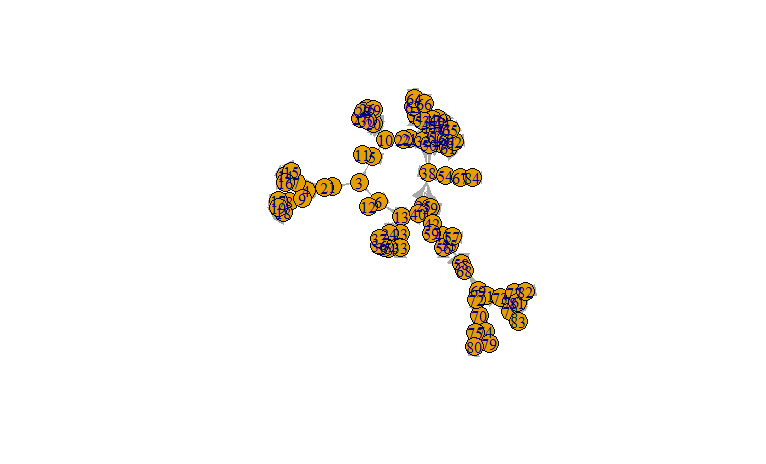
\includegraphics[width =  0.7\textwidth]{plots/network_vietnam.png} 

\item Avantages : description fine des échanges (quantités, occasion, type de relation... )

\end{itemize}
\end{frame}
%-------------------------------------------------------------------------------

\begin{frame}{Encodage en matrice}
\begin{itemize}
\item Définir un tableau avec en ligne et en colonne les individus. 
\item Dans chaque case $(i,j)$ : 
$$y_{ij} =
\left\{ 
\begin{array}{cl} 1&  \mbox{ si relation entre $i$ et $j$}\\

 0 & \mbox{ sinon}
 \end{array}
 \right.$$ 
 
{ \centering
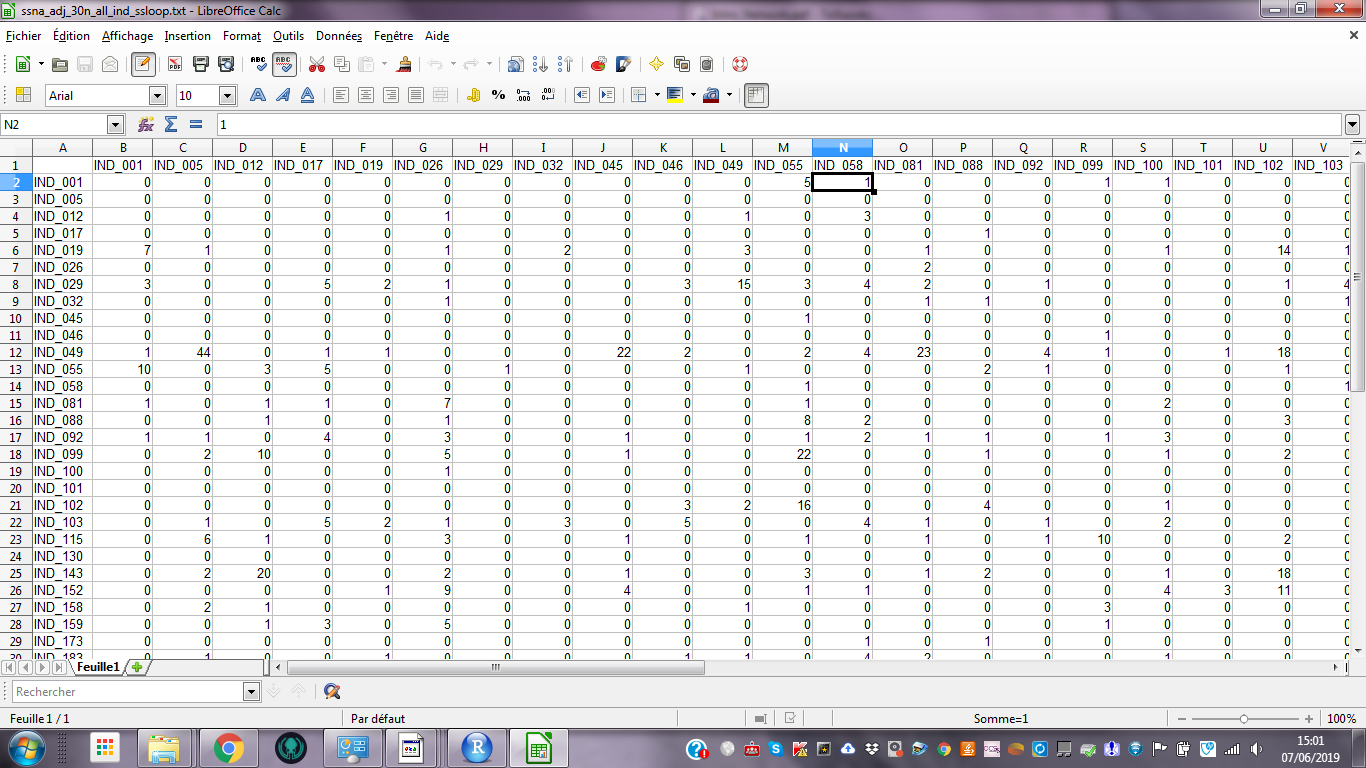
\includegraphics[width =  0.6\textwidth]{plots/ecran_data_vanuatu.png}\\
}
(données du Vanuatu)
\item Passage de liste d'arête à la matrice d'adjacence/incidence par une fonction \textsf{R} : \textsf{igraph}
\item Ne permet pas de stocker les descripteurs de la relation. 
\end{itemize}
\end{frame}
%-------------------------------------------------------------------------------


\begin{frame}{Dessin de la matrice}
Représentation de cette matrice : une case noire   $ \neq 0$
\vspace{1em}

{\centering
\begin{tabular}{cc}
 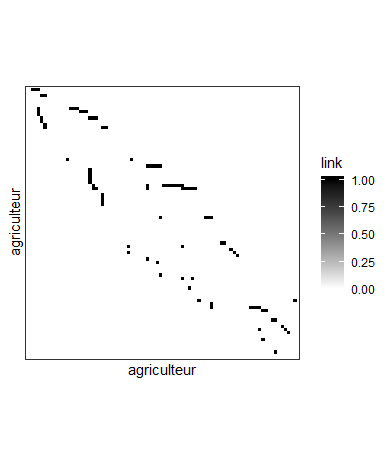
\includegraphics[width =  0.35\textwidth]{plots/matrix_vietnam.png} & 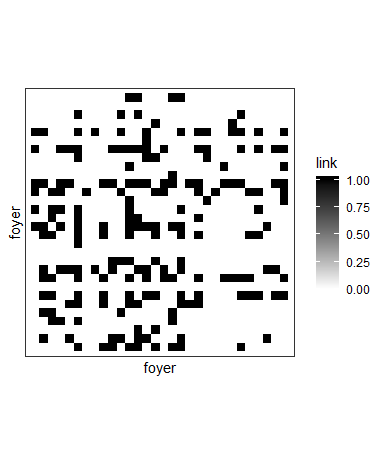
\includegraphics[width =  0.35\textwidth]{plots/Vanuatu_matrix.png}\\
\hline 
Vietnam & Vanuatu \\
\hline 
 \end{tabular}}
 
 \end{frame}
 



%-------------------------------------------------------------------------------
\section{Les différents types de réseaux}





\begin{frame}{Les réseaux simples}

\begin{itemize}

\item Relation au sein d'un groupe d'acteurs :  amitiés, échange de semences, co-occurrences d'espèces, réseaux trophiques
\begin{itemize}
\item Matrice d'adjacence : matrice carrée
\end{itemize}

\end{itemize}
\end{frame}
%----------------------------------------------------------- 
\begin{frame}{Les réseaux dirigés ou non}

\begin{center}
Relation peut être \emph{orientée (dirigée)} ou non
\end{center}


\begin{tabular}{ccc}
\hline
& \textbf{Réseaux orientés} & \textbf{Réseaux non-orientés}\\
\hline
Exemples &  Don,  réseau trophique & Amitiés, co-occurence d'espèces\\
\hline
Arête & flèche & trait\\
\hline
Matrice  & carrée, non-symétrique& carrée, symétrique\\
& $y_{ij} \neq y_{ji}$ & $y_{ij} = y_{ji}$\\
\hline
\end{tabular}
 
%\begin{columns}
%\begin{column}{0.5\textwidth}
%\centering{} 
%\begin{itemize}
%\item  : 
%\item  : flèche
%\item d'adjacence : 
%$$X_{ij} \neq  X_{ji}$$
%\end{itemize}
%\end{column}
%\begin{column}{0.5\textwidth} 
%\centering{\textbf{Réseaux non-orientés}} 
% \begin{itemize}
%\item \emph{Exemples : 
%\item \emph{Arête : trait
%\item \emph{Matrice d'adjacence : carrée, symétrique
%$$X_{ij}=  X_{ji}$$
%\end{itemize}
%\end{column}
%\end{columns}

\end{frame}
%
%
%%----------------------------------------------------------- 
%\begin{frame}{Exemple en écologie: coexistence d'espèces, relation non dirigée  }
%
%
%\begin{itemize}
%\item Sommets : espèces 
%\item Relation : coexistence 
%\item Arête entre espèces $i$ et $j$ si les deux espèces coexistent
%
%\item Encodage 
%$$ X_{ij} = X_{ji} = \left\{ \begin{array}{cl} 0& \mbox{si pas d'arête} \\ 1 & \mbox{sinon} \end{array} \right. $$   
%\end{itemize}
% 
%
%\end{frame}
%
%\begin{frame}{Exemples en écologie : relations   dirigées}
%\centering
% 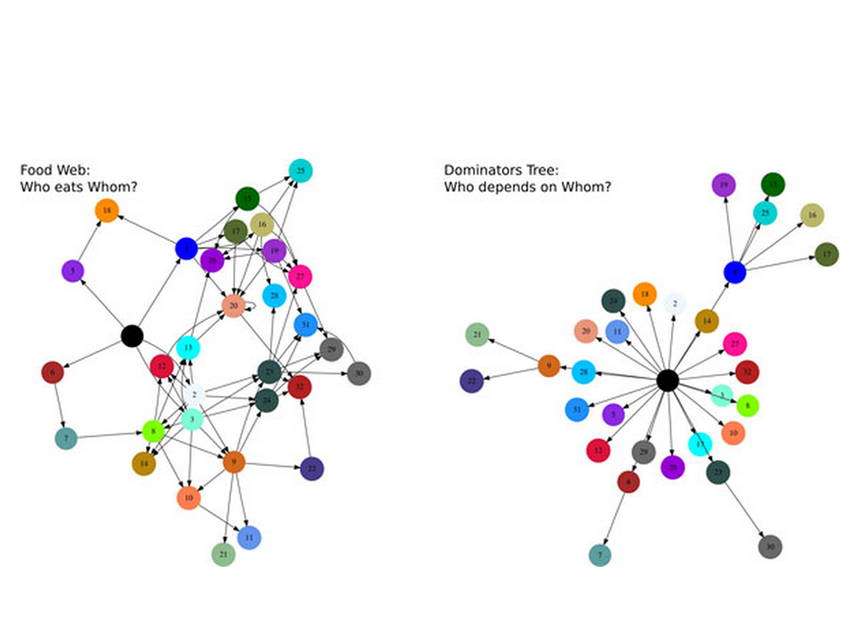
\includegraphics[width = \linewidth]{plots/ecological_network_general.png}
%
%\end{frame}
%
%
%
%
%%-------------------------------------------------------------------------------
%\begin{frame}{Exemple:  circulation de graines, relation dirigée  }
%
%
% 
%\begin{itemize}
%\item Sommets : foyers 
%\item  Relation : échange de semences 
%\item Arête (flèche) de $i$ vers $j$ si $i$ donne des semences à $j$. 
%\end{itemize}
% 
% \begin{tabular}{cc}
%  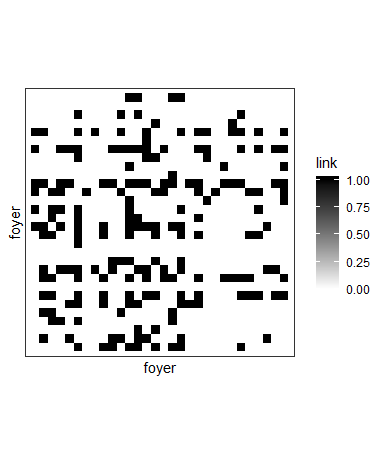
\includegraphics[width = 5cm]{plots/Vanuatu_matrix.png} &
% 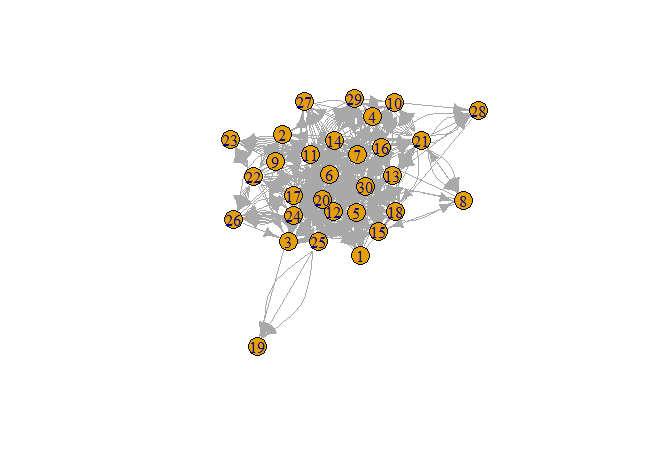
\includegraphics[width = 5cm]{plots/Vanuatu_directed.png}
%\end{tabular}
%\vspace{-2em}
%$$ \begin{array}{ccl}
% X_{ij}  &=& \left\{ \begin{array}{cl} 1& \mbox{si $i$ donne à $j$} \\ 0 & \mbox{sinon} \end{array} \right. \\
%\end{array} \quad X_{ij}   \neq   X_{ji}$$
%
%
%
%\end{frame}
%
%%-------------------------------------------------------------------------------
%\begin{frame}{Exemple: circulation de graines, relation dirigée  et valuée}


%----------------------------------------------------------- 
\begin{frame}{Les réseaux valués}

La relation peut être décrite par un nombre, orientée ou non. 

\begin{itemize}
\item Exemple : nombre de fois où $i$ a donné des semences à $j$
\item Arête : épaisseur du trait proportionnelle à la valeur
\item Matrice : symétrique ou non, pas seulement de $0/1$
\item $y_{ij} \in \mathbb{N}$, $y_{ij} \in \mathbb{R}$  
\end{itemize}

\end{frame}


 


%-------------------------------------------------------------------------------
\begin{frame}{Réseaux bipartites}

\begin{block}{Définition}

Un réseau est dit bipartite si les sommets sont divisés en deux sous-ensembles et  une arête a une extrémité dans un des sous-ensemble et l'autre dans l'autre sous-ensemble. 
\end{block}
\begin{center}
   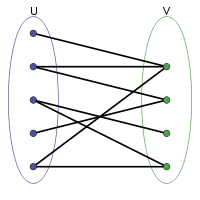
\includegraphics[width =0.3\linewidth]{plots/Simple-bipartite-graph.png}
\end{center}
\end{frame}




%-------------------------------------------------------------------------------
\begin{frame}{Exemple de réseau bipartite: inventaire de cultures}

\begin{itemize}
\item  Entre de sommets $U$: foyers
\item  Entre de sommets $V$:  espèces végétales
\item  Relation : culture 
\item Arête entre $i$  et $j$    si foyer $i$ cultive espèces $j$. 
\end{itemize}
 

 \begin{tabular}{cc}
  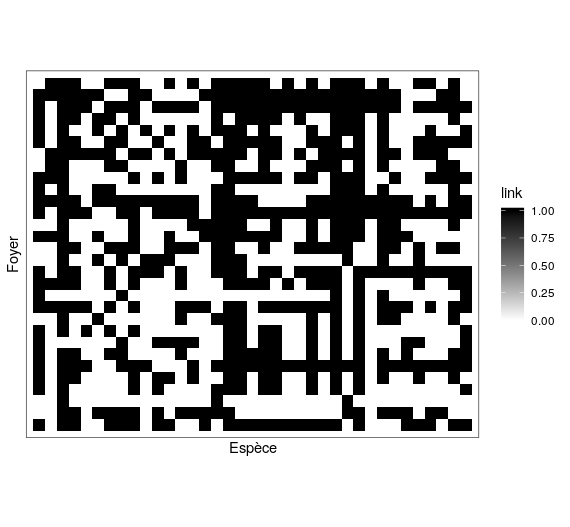
\includegraphics[width = 5cm]{plots/Vanuatu_incidence.png} &
 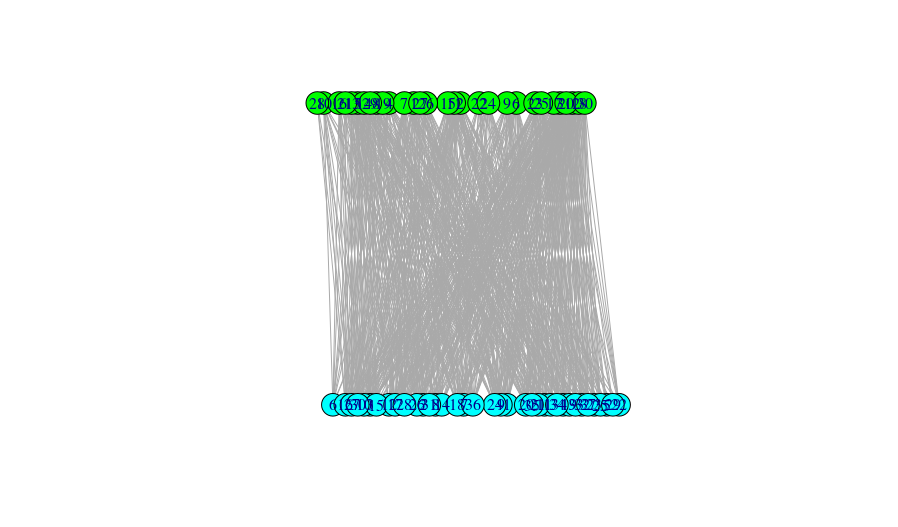
\includegraphics[width = 8cm]{plots/Vanuatu_bipartite.png}
\end{tabular}


\end{frame}

%----------------------------------------------------------------------- 
\section{Inférence statistique}


\begin{frame}{Statistiques : pour quoi faire? }

Comprendre ça: 
\centering
 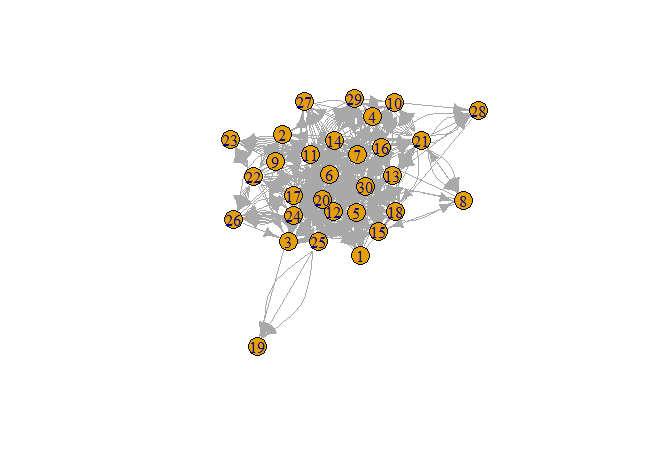
\includegraphics[width =  \textwidth]{plots/Vanuatu_directed.png}  

\end{frame}


\begin{frame}{Statistiques : pour quoi faire? }


\begin{block}{Comprendre / étudier la structure du réseau}
\begin{itemize}
\item Vue générale :  
\begin{itemize}
\item très connecté  / peu connecté (densité)...  
\item Existence de star?  
\item Communauté (= sous-groupes d'acteurs plus connectés entre eux qu'avec le reste des acteurs).   
\end{itemize}
\item Du point de vue des individus : existence de  généralistes et de spécialistes,  centralité, etc.. 
\item Avoir une vue résumée du réseau
\end{itemize}
\end{block}
\end{frame}


%-------------------------------------------------------------------------------
\begin{frame}{Comment faire?}
\begin{block}{Si le réseau est petit (10-15 sommets)...}
Possible de le faire à la main


\end{block}

\begin{block}{Si plus de sommets... }

\begin{itemize}
\item Statistiques descriptives 
\item Approche egocentrée 
\item Modèles probabilistes : modèles à blocs stochastiques
Outils automatiques pour faire des groupes de sommets qui ont le même rôle dans le réseau 
\end{itemize}

\end{block}
\end{frame}


%
%\begin{frame}[allowframebreaks]{Références}
%\bibliographystyle{apalike}
% \small{ \nocite{*}
%\bibliography{biblio}}
%  \end{frame}
%  
  
  
\end{document}
